\section{Models}

\subsection{the tendency of language speakers}
\noindent There are two keys to be considered about the language trends: the change in the number of language speakers and their geographical distribution. The key to studying the change in the number of speakers is to build a sound predictive model. Considering the incompleteness and roughness of the statistical data about speakers, we consider the establishment of a non-equidistant gray prediction model. In considering the geographical distribution of language speakers, we study the following two aspects: the regional disparities in the distribution of the language speakers in different regions and the changes in the geographical distribution of second languages due to immigration.

\subsubsection{Changes in the number of language speakers}
\noindent For the study of the trend of global language change, we should consider two aspects, that is, the change in the total population of a certain language and the change in geographical distribution of language speakers, As explained in the Problem Analysis, when predicting trends in the population of languages, we first need to collect historical data about the particular language being used.The data are listed below:


\begin{table}[H]
	\centering
	\caption{Global rankings in 2014, 2015, 2016, 2017 Change in total headcount usage in the top 23 languages}
		 \scalebox{0.87}[0.87]{%
	\begin{tabular*}{35em}{@{\extracolsep{\fill}}clrrrr}
		\toprule
		\multicolumn{1}{l}{Number} & Language & 2014  & 2015  & 2016  & 2017 \\
		\midrule
		1     & Chinese,Mandarin & 1052.535 & 1070.966 & 1073.525 & 1076.734 \\
		2     & Spanish & 441.7462 & 453.7809 & 466.8536 & 480.4602 \\
		3     & English & 816.9127 & 903.37 & 911.6737 & 917.9667 \\
		4     & Hindi & 365.4672 & 365.735 & 366.4932 & 367.5688 \\
		5     & Portuguese & 196.7223 & 198.126 & 200.7203 & 202.5036 \\
		6     & Bengali & 184.1833 & 186.2771 & 183.2275 & 179.4995 \\
		7     & Russian & 189.6124 & 192.1039 & 194.2471 & 197.3681 \\
		8     & Japanese & 124.9867 & 125.1537 & 125.3209 & 125.5303 \\
		9     & Javanese & 77.36284 & 76.93927 & 76.51803 & 75.99483 \\
		10    & German,Standard & 146.0954 & 146.6092 & 147.6057 & 148.2428 \\
		11    & Chinese,Wu & 73.22911 & 72.48929 & 71.75694 & 70.85228 \\
		12    & Korean & 117.8224 & 117.8665 & 117.9106 & 117.9658 \\
		13    & French & 126.9646 & 153.8068 & 154.9492 & 155.939 \\
		14    & Telugu & 81.37525 & 81.70919 & 82.14315 & 82.18562 \\
		15    & Marathi & 71.41339 & 71.47918 & 71.54502 & 71.62742 \\
		16    & Turkish & 58.45415 & 58.32959 & 58.2053 & 58.05032 \\
		17    & Tamil & 73.58453 & 73.5565 & 73.52849 & 73.4935 \\
		18    & Vietnamese & 67.34071 & 67.26303 & 67.18545 & 67.0886 \\
		19    & Urdu  & 153.8177 & 153.5716 & 153.3494 & 153.0674 \\
		20    & Italian & 64.94941 & 64.9459 & 64.94238 & 64.93799 \\
		\bottomrule
	\end{tabular*}%
}
	\label{tab:addlabel}%
\end{table}%

 The table above shows the changes in the total number of people speaking the top 23 languages in the world in 1999, 2009, 2014, 2015 and 2017.
 
 We analyze the data in the above table and consider the small amount of data (only four years of data), while the Gray Prediction Model has the characteristics of less input data but high prediction accuracy. And driven by reference\upcite{gray}, we establish a non-equidistant Gray Prediction Model GM (1,1) to predict the number of language speakers.Due to the non-equidistant distribution of data over time, we define non-equally spaced sequences of language speakers:



\begin{equation}
\begin{aligned}
& {x_j}^{(0)}({k_i}) = \left\{ {{x_j}^{(0)}({k_1}),{x_j}^{(0)}({k_2}),...,{x_j}^{(0)}({k_n})} \right\} ,\\
& \qquad \qquad \qquad \Delta {k_i} = {k_i} - {k_{i - 1}} \\
\end{aligned}
\end{equation}
\noindent
where, ${x_j}^{(0)}({k_i})$ represents the sequence of changes in the number of speakers in the m-th language over time, ${x_j}^{(0)}({k_n})$  is the total number of people who speak the $j$-th language in ${k_i}$ year ,(where n = 4), which corresponds to four years in the historical data. Obviously $\Delta {k_i}$  is not a fixed value here. Because we have only four sets of data, which contains very little system information,. In order to strengthen its regularity, we will do Accumulated Generating Operation on it, the result of a cumulative sum is defined as AGO of the non-equally spaced sequence ${x_j}^{(0)}({k_i})$ , marked as

\begin{equation}
{x_j}^{(1)}{\rm{(}}{k_i}{\rm{) = }}\left\{ {{x_j}^{(1)}({k_1}),{x_j}^{(1)}({k_2}),...,{x_j}^{(1)}({k_n})} \right\},\label{aa1}
\end{equation}
\noindent
Where ,  makes the following formula true 

\begin{equation}
{x_j}^{(1)}{\rm{(}}{k_i}{\rm{) = }}\sum\limits_{m = 1}^i {{x_j}^{(0)}({k_j})\Delta {k_j}{\rm{ ,  }}} i = 1,2,...,n. 
\end{equation}

Based on the above, the steps of using non-equidistant Gray Prediction Model\upcite{gm11} to predict the number of speaking speakers over the next 50 years are as follows:

 \begin{enumerate}
 \item[\textbf{Step1}]  Determine the interval of non-equally spaced sequences.
 \item[\textbf{Step2}] From the formula (1) to generate a cumulative sequence.
 \item[\textbf{Step3}] Least square method is used to determine the parameters a\&b to be identified in the albinism differential equation ,that is
		 \begin{equation}
		 \phi {\rm{ = }}\left[ {\widehat a\widehat b} \right] = {({B^T}B)^{ - 1}}{B^T}Y ,
		 \end{equation}
		 
	where, $B{\rm{ = }}\left[ {\begin{array}{*{20}{c}}
		{{z_m}^{(1)}({k_1})}1\\
		\vdots  \vdots \\
		{{z_m}^{(1)}({k_n})}1
		\end{array}} \right]$, $Y{\rm{ = }}({x_j}^{(0)}({k_2})\Delta {k_2},{x_j}^{(0)}({k_3})\Delta {k_3}, \cdots ,{x_j}^{(0)}({k_n})\Delta {k_n})$ and ${z_j}^{(1)}({k_i})$  is the background value \upcite{influential} of ${x_j}^{(1)}(t)$  on the discrete interval  $\left[ {{k_i},{k_{i + 1}}} \right]$.
  \item[\textbf{Step4}] The estimate ${\widehat x_m}^{(0)}({k_{i + 1}})$ of ${x_m}^{(0)}({k_{i + 1}})$  is calculated\upcite{influential} from the parameters a, b.
\end{enumerate}

From the above derivation process, we use MATLAB (Programming code is shown in appendix) as a programming tool to determine the total number of the mainstream languages speakers in the next 10 years the results( Figure \ref{fig:next50}) are as shown below:
     

\begin{figure}[H]
	\centering
	 \scalebox{0.87}[0.87]{%
	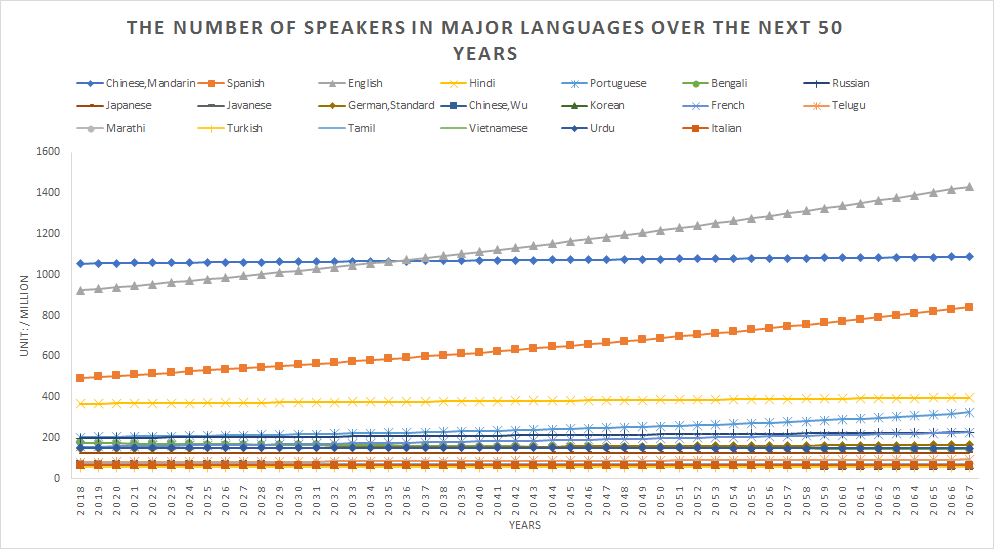
\includegraphics[width=1\linewidth]{figures/next50number}
}
	\caption{The number of speakers in major languages over the next 50 years}
	\label{fig:next50}
\end{figure}

After analyzing the figure above, we find that the total number of English-speaking population exceeded that of Chinese by 2045 and become the most heavily spoken language in the world.Additionally, the most powerful growth is in Spanish. In 2067, the rankings of the top ten mainstream languages in the world are:

\textbf{English,Chinese Mandarin, Spanish ,Hindustani, Arabic ,Portuguese, Russian, French, German Standard, Malay.}

The changes in the number of native speakers in the future areshown in the following Figure \ref{fig:percent1} :
\begin{figure}[H]
	\centering
	 \scalebox{0.87}[0.87]{%
	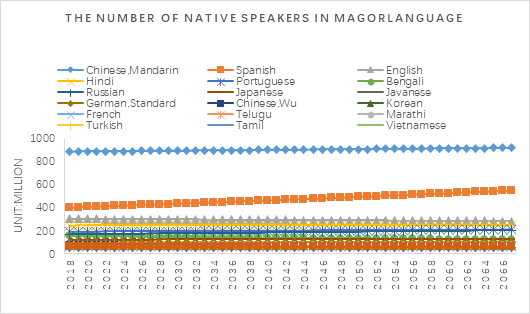
\includegraphics[width=1\linewidth,,height=8.1cm]{figures/percent}
}
	\caption{The number of native speakers in major language}
	\label{fig:percent1}
\end{figure}
Analyzing the figure above, we find that the number of people who speak Mandarin as their mother tongue is the largest, followed by Spanish, with the most pronounced growth trend in the language. In 2067, the top 10 languages that are speaked as the first languages are Chinese Mandarin, Spanish, English, Hindi, Portuguese, Arabic, Bengali, Russian, Japanese, German Standard.

Considering the results of the analysis of the above two graphs and comparing the current two rankings provided in the topic, we can get the following table (Table \ref{tab:Language}):


% Table generated by Excel2LaTeX from sheet 'Sheet1'
\begin{table}[H]
	\centering
	\caption{Language ranking comparison}
	 \scalebox{0.87}[0.87]{%
	\begin{tabular}{l p{2.8cm}p{2.8cm}p{2.8cm}p{3.2cm}}
		\toprule
		\multicolumn{1}{l}{Rank} & native speakers(2017 year) & native speakers(2067 year) & total speakers(2017 year) & total speakers(2067 year) \\
		\midrule
		1     & Mandarin & Mandarin & Mandarin & English \\
		2     & Spanish & Spanish & English & Mandarin \\
		3     & English & English & Hindustani & Spanish \\
		4     & Hindustani & Hindustani & Spanish & Hindustani \\
		5     & Arabic & Portuguese & Arabic & Arabic \\
		6     & Bengali & Arabic & Malay & Portuguese \\
		7     & Portuguese & Bengali & Russian & Russian \\
		8     & Russian & Russian, & Bengali & French, \\
		9     & Punjabi & Japanese & Portuguese & German,Standard \\
		10    & Japanese & German Standard. & French & Malay \\
		\bottomrule
	\end{tabular}%
}
	\label{tab:Language}%
\end{table}%

Our analysis of top 10 languages in 2017 and 2067 shows the following results: it is true that none of the top ten languages are replaced for both native speakers and total speakers , but the exact rankings of the ten languages change. The total number of English speakers surpassed that of Chinese. In the mother tongue, Chinese still occupy the dominant position, followed by Spain to maintain the status of second place unchanged.

\subsubsection{The impact of Population Migration on the Geographical}
\noindent
Simulating the geographical distribution of changes in the population of different languages, we consider two key factors: the change in the number of languages in the world and the immigration situation. For the former, we compare the difference in the number of the same language speakers in different regions. In that way, we obtain the transformation law of geographical distribution of the population speaking the language.And for the latter,a population-flow model is proposed to simulate immigration, which can show the change of the geographical distribution of the language caused by immigrants over time. To facilitate modeling, as described in the problem analysis, we define Asia, Europe, Africa, North America, South America, and Oceania as the six-language collective, Respectively marked as ${R_1},{R_2}, \cdots ,{R_m}$ ,where m is 6 . According to reference \upcite{gm11}, we find that more than half of the world's growing population over the next 50 years is derived from Africa. And given our time constraints, we study only in the top 20 languages in Africa (the region most likely to be the center of distribution for language speakers. Based on the results calculated from the model built in the first part of the question we chose French, Italian, Arabic, English, Portuguese as the research object.

In order to facilitate the analysis of the geographical distribution of a linguistic population over time,we define language regional collective as follows:

\begin{equation}
{\gamma _i} = \frac{{L{1_i}^j}}{{\sum\limits_{i = 1}^6 {L{1_i}^j} }},
\end{equation}
\noindent
${\gamma _i}$ characterizes the degree of distribution of a language in a Language Regional Collective,.The greater the value, the greater the number of speakers of that language in this region.

After that, we compare the values of ${\gamma _i}$ in different regions and then we can get the geographical distribution differences of the studied languages.

Apply ing the data from the first part of the modeling (see Annex 1), we can get the change of the ratio of the total speakers of French, Arabic, Italian, English and Portuguese to the total speakers in these four languages in Africa. The results are shown in the following figure.

\subsubsection{Impact of Population Migration on the Geographical Distribution of Second Language}
\noindent Based on the above questions, we can draw a conclusion that the number of second language speakers in the number of changes in the trend because the world outside the mother tongue of a second language is known geographical map, combined with Google Maps Analysis of the second language used mainly as follows(The figure below is part of the data. See the attached Table \ref{tab:SixContinents} for all the data.):

% Table generated by Excel2LaTeX from sheet 'Sheet2'
\begin{table}[H]
	\centering
	\caption{ The second language is mainly used in countries / regions}
	 \scalebox{0.8}[0.8]{%
	\begin{tabular}{llp{6cm}p{6cm}}
		\toprule
		language & Asian & Europe & Oceania \\
		\midrule
		Chinese &       &       & Australian \\
		\midrule
		English &       & Sweden, France, Iceland, Poland &  \\	\midrule
		spanish &       &       &  \\	\midrule
		Arabic &       &       &  \\	\midrule
		Russian &       &Ukraine, Kazakhstan, Uzbekistan,Turkmen&  \\	\midrule
		Bengalese & India&       &  \\	\midrule
		Portuguese &       &       &  \\	\midrule
		French &       &       &  \\	\midrule
		Hausa &       &       &  \\	\midrule
		Turkish &       & Austria,Germany, Bulgaria &  \\	\midrule
		Italian &       &       &  \\
		\bottomrule
	\end{tabular}%
}
	\label{tab:addlabel}%
\end{table}%

\par According to the above table and the relevant data \upcite{travel}, we can see that as the top10 of the second language of the country, the following are arranged in order (in parentheses, the number of countries): English (55), French (14), Russian (13), Spanish , Creole (8), Arabic (8), Kurdish (4), Portuguese (4), Italian (3), Quechua (3).
\par The changes in the geographical distribution of the second language mainly consider the impact of the population migration pattern, in which the migration pattern of the population is mainly influenced by government policy and emigration of a country. We simply think that no government intervention or intervention policy in a certain period of time remained basically unchanged, so we only consider the impact of immigration factors on the second language in the geographical distribution of change.According to the data, we choose to use the net migration to reflect the immigration factor. It is known that the United Nations predicts the net migration before 2100 \upcite{undata}, and at the same time it can avoid errors in the data obtained by our own prediction model.To simplify the model, we assume that the net number of new moves in a given linguistic region is proportional to the number of new speakers using the dominant language in the region as a second language,and the definition of the newly added population that dominates the region's second language as an assimilated population.
\par We can calculate the number of people who are assimilated in the language region by the number of net immigrants in a language region. As follows:

\begin{equation}
\L2_i^j{\rm{ = }}\frac{{P_i^j}}{{\sum\limits_{i = 1}^n {P_i^j} }}L{2^j},\label{aa1}
\end{equation}

\noindent Among them: $P_i^j$ represents the number of net immigrants in a country's second language, $L2_i^j$ represents the number of assimilated people in a certain language region, that is, the number of second-language growers, $L{2^j}$ represents the $j$th-language growth,this value is determined by the model of the first part of the question.
\par According to the above analysis and formula, Echarts Gallray can be used to make a dynamic map of the geographical distribution of a second language under the influence of population migration \upcite{mapdata}. The geographical distribution of second language speakers in each language in the above table can be displayed.Random screenshots here to get the number of speakers in English, Spanish as a second language in the geographical distribution of changes:

\begin{figure}[htbp]
	\centering
	 \scalebox{0.87}[0.87]{%
	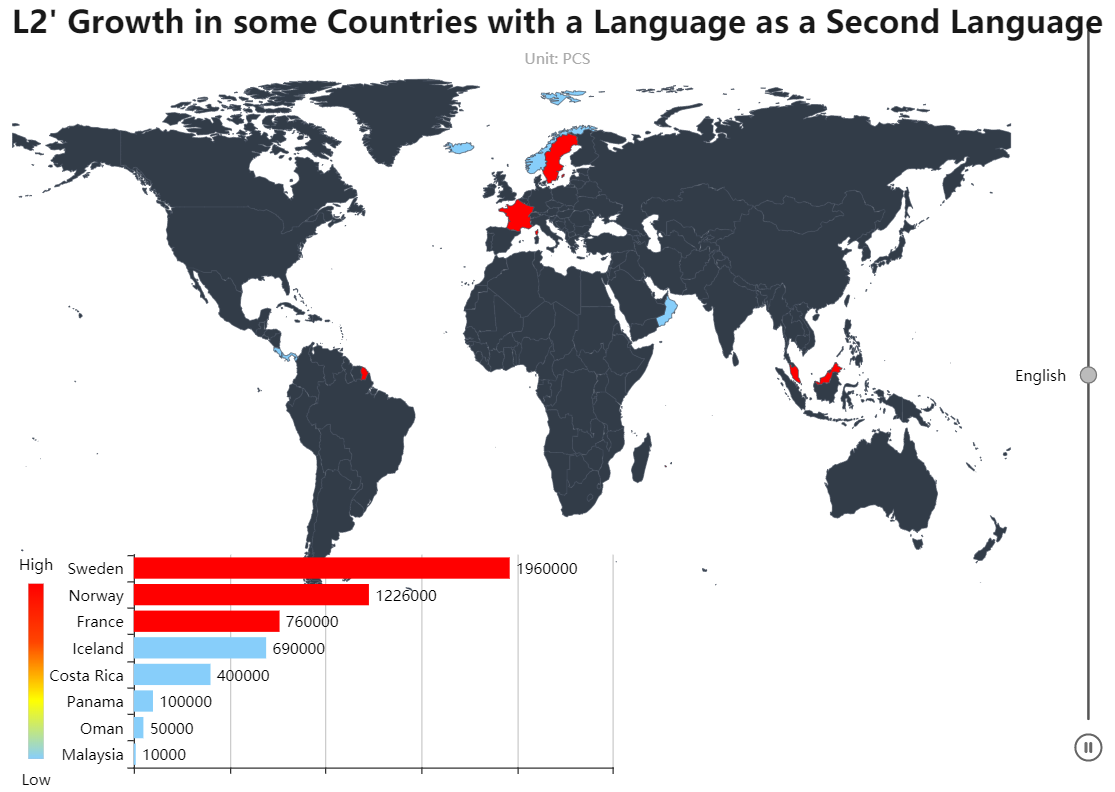
\includegraphics[width=1\linewidth,height=10cm]{figures/english}
     }
	\caption{Geographical distribution of English as a second language in 2067}
	\label{fig:english}
\end{figure}

\noindent Note: The color column changes upward, representing the increase in the number of more.

 From the comparison between the above figure and the known geographical distribution in 2017, we can see that the countries currently speaking English as the second language are mainly located in four regions:Western and Central European countries (Sweden, Norway, France, Iceland, Poland), Malaysia, Central American countries, East African countries (Egypt, Sudan, Cameroon).The number of L2 speakers in English in 2017 was 611 million, rising to 1.147 billion in 2067, an increase of 536 million in the number of speakers of L2 in 50 years.Of these, countries rank the highest to the lowest in the country: 1,976,000(Sweden)> 1,226,600(Norway)> 76,000(France)> 69,000 (Iceland) > 400,000 (Costa Rica) > 100,000.
\par Analysis of the geographical distribution of changes:
\begin{itemize}
	\item The growth of the three North West European countries, Switzerland, Norway and France, showed the most noticeable changes. The growth rates of these three countries were all above 700,000. In addition, some Nordic countries also saw an increase in their numbers;
	\item The number of Central American countries and the Malay archipelago has been significantly reduced;
	\item African countries have a net negative net migration, so few people have used English as their second language. 
\end{itemize} 

\par The figure below is the geographical distribution of Spanish as a second language:

\begin{figure}[htbp]
	\centering
	 \scalebox{0.87}[0.87]{%
	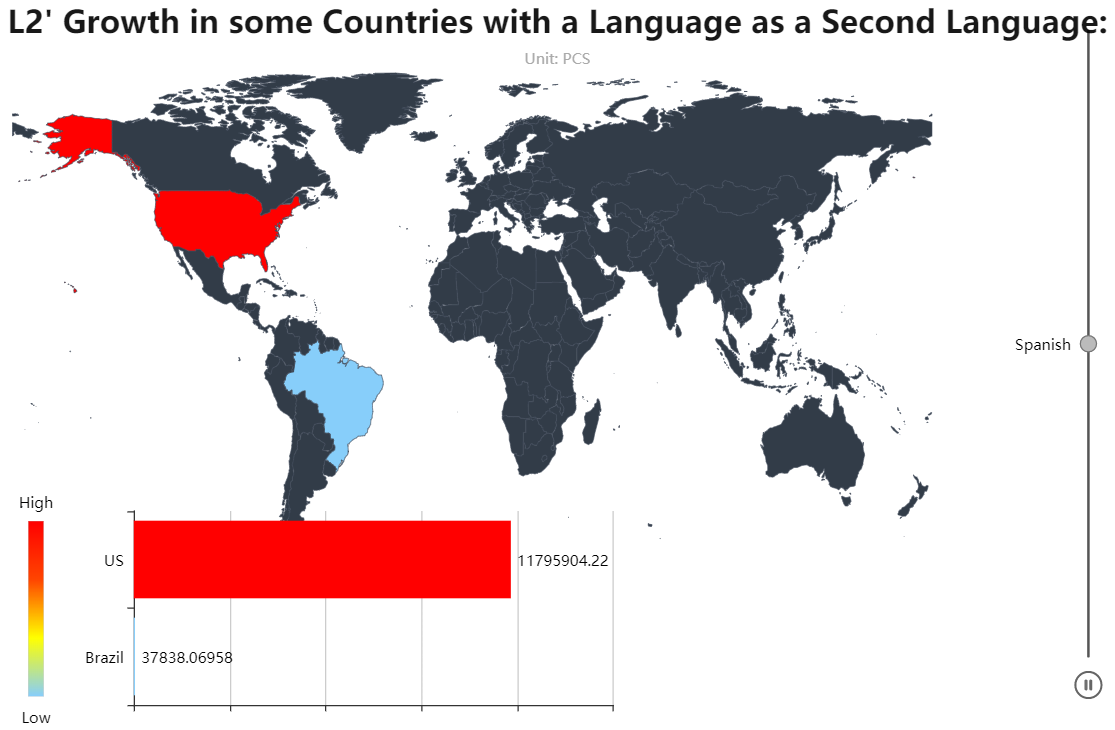
\includegraphics[width=1\linewidth,height=10cm]{figures/Spanish}
}
	\caption{Geographical distribution of Spanish as a second language in 2067}
	\label{fig:spanish}
\end{figure}

\par From the above figure and the known geographical distribution in 2017, we can see that: Currently, countries with Spanish as their second language are mainly based on estimates in the United States and Brazil. The number of L2 users in Spain by 2067 was 152 million, an increase of 62 million compared with 90 million in 2017. Affected by the number of net immigrants, the migration to the United States is about 11.7 million more than that of Brazil, so the color shown in the United States is red and the color shown in Brazil is light blue. 

\subsection{the location of the new international office}

\noindent Effective language can promote the development of business, so we consider choosing to develop the company's business in a region where language has potential for development. Based on the results of the first part of the question, we build a model of linguistic performance evaluation that evaluates and ranks the performance of languages to determine the preferred locations for the six international offices.

\par First of all, we need to determine the evaluation index to build the evaluation model.The evaluation indicators are selected from the five categories of geography, economy, total number of languages spoken in one language (inc.pl1 \& pl2), information output and quality of languages, and the situation in which the international organizations use the language.We consider that many of the indicators are economic-related and not directly related to language.Therefore, we think that the indicator of the economy is directly related to the dominant language of the economy. What needs to be pointed out is that for a certain language we only count the countries where the native language is in this language and the population exceeds 10million.
\par Then, as explained in the Problem Analysis section, we set up a language performance evaluation (L\,I\,I) model.Taking into account that the indicators have different dimensions, we quantify each indicator to [0,1], calculate the language influence score and rank them. According to the rankings, the cities were specifically identified based on the state of the economy at the national level in the language and the reasons for the changes in the locations of the six new international offices in the short and long term were analyzed.Finally, consider the changes in the nature of global communications, the widespread use of electronic media, more and more convenient and accurate translation software, making language constraints reduced,multinational corporations may consider opting to set up offices in less than six places, giving the location of the office and describing the corresponding reasons.

\subsubsection{Language Effectiveness Evaluation Model((L\,I\,I) } 

\noindent In order to evaluate the linguistic influence more reasonably, we have been inspired by reference\upcite{influential} to propose the language influence Index (L\,I\,I) model.Language Influence Index (L\,I\,I) selects 14 indicators to measure the influence of language from 5 aspects. The 14 indicators we choose are as follows:

\begin{enumerate}
	\item[1)] \textbf{Area: Extensive geographical advantage of language diffusion}
	\par \textbf{Number of countries that speak the language :}This indicator relates to the number of countries or regions that use this language as their mother tongue and some also include this language as a second language.The greater number of countries that use this language as a mother tongue or a second language demonstrates that the distribution of language is more adequate and the greater the international influence of the language.We define the mapping rules for this metric as follows: If a language is "dominant", the metric is valued of 1; conversely, if it is a "minority", its value is 0.5.
	\par \textbf{National Land area:}By looking at the data\upcite{influential}, we know that the size of the land area can be approximated to measure a country's linguistic exclusiveness, which in turn affects the country's "dominant" language's international influence.
	\par \textbf{Inbound tourists:}This indicator mainly reflects the number of overnight visitors to the country. Mainly by the language group's culture to attract, and understand a culture must learn the culture carrier language.
	\par \textbf{National Land area:}By looking at the data [7], we know that the size of the land area can be approximated to measure a country's linguistic exclusiveness, which in turn affects the country's "dominant" language's international influence.
	\par \textbf{Inbound tourists:}This indicator mainly reflects the number of overnight visitors to the country. Mainly by the language group's culture to attract, and understand a culture must learn the culture carrier  language.
	
	\item[2)] \textbf{Economy strength: Language plays an important role in economic life}
	\par \textbf{GDP: }The level of economic development of a language group has an obvious and self-evident important influence on the international influence of the language. Therefore, we include it in the indicator range.
	\par \textbf{GDP per capita:}This indicator reflects the overall level of development of a region and can characterize the attraction of the region to those who have the will to emigrate.
	\par \textbf{Exports: }When exports are larger than imports, trade surpluses often appear and trade surpluses can enhance the international influence of regional languages.
	
	\item[3)] \textbf{Language speakers: Direct Impact factors}
	\par \textbf{Native speakers and Second language (L2) speakers:} These two indicators are based on the first part of the forecasting model, and have a direct impact on the linguistic impact assessment and analysis.
	
	\item[4)] \textbf{Knowledge and media: An important channel for language communication}
	\par\textbf{Internet use language: } The Internet has an important influence on the spread of language influence. With the globalization of information, the possession of a language in the Internet plays an important role in developing the international influence of the language.
	\par \textbf{Higher education uses language:}The language used in a national education and teaching school, especially the language used in higher education, and outstanding education will attract a large number of overseas students and thus promote the conversion of a foreign language into a second language.
	
	\item[5)] \textbf{International use: Language in the international recognition}
	\par \textbf{International organizations:}We consider that some international organizations in the world play an important role in promoting the spread of linguistic influence. Therefore, we think the index as a measure. Here we consider the IMF, UN, WB and other 10 international organizations (index of 10 organizations).For example, if a language is the official language of the International Monetary Fund, the indicator picks up the value of 1, otherwise 0. From Wikipedia, you can find the official language used by each international organization.
	
\end{enumerate}

\par To show the structure of our model more clearly, here's a diagram of the Language Influence Index (L\,I\,I):

\begin{figure}[htpb]
	\centering
	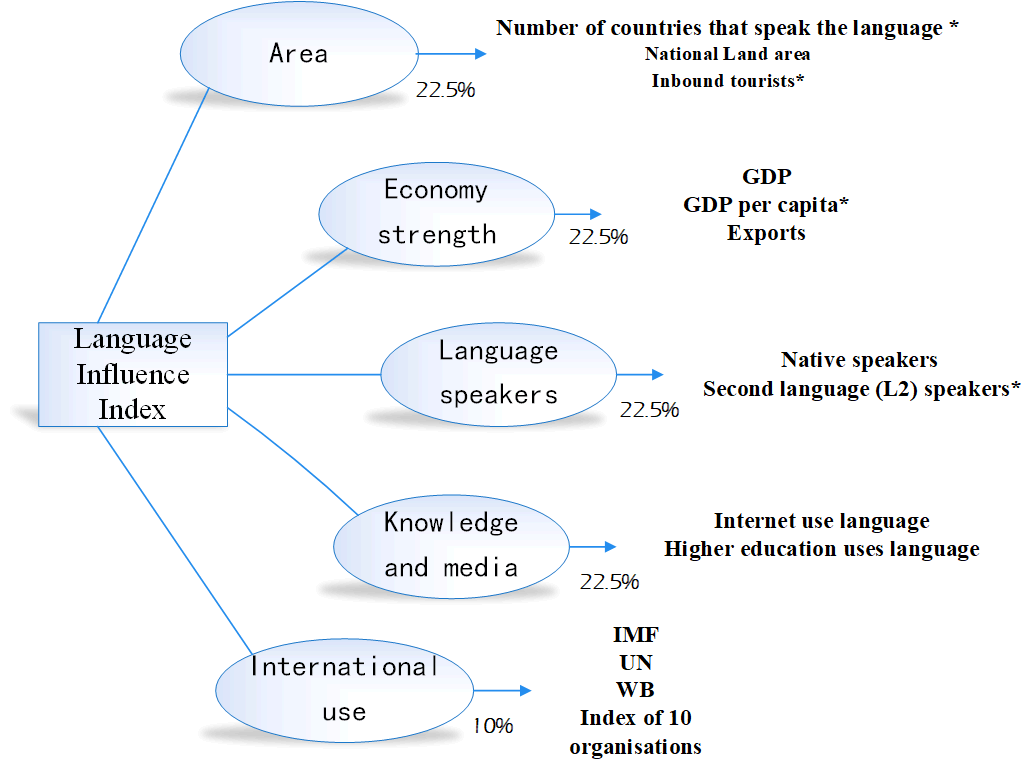
\includegraphics[width=0.7\linewidth]{figures/chart}
	\caption{Language Influence Index Structure chart}
	\label{fig:chart}
\end{figure}

\par \textbf{L\,I\,I model construction process is as follows:}

\begin{enumerate}
	\item[1)] \textbf{Determination of the weight of influence index}
	\par Assuming that the overall weight of the indicator is 1, when considering the five aspects of the promotion of the international influence of the language, the indicators in the first four categories together account for 0.9, and the weight in the final category accounts for 0.1. At the same time, the weight of indicators in each aspect is inversely proportional to the number of indicators.The definition uses ${\omega _m}$ for the weight of each indicator and $m$ for the mth indicator:



		\begin{equation}
	{\omega _m} = \left\{ \begin{array}{l}
	\frac{{0.9}}{4} \times \frac{1}{3} = 0.075{\rm{          }} \qquad m = 1,2,3{\rm{ ,4,5,6 }}\\
	\\
	\frac{{0.9}}{4} \times \frac{1}{2} = 0.1125{\rm{        }}\qquad m{\rm{ = }}7,8,910\\
	\\
	0.1 \times \frac{1}{4} = 0.025{\rm{           }}\qquad m = 1112,13,14
	\end{array} \right.
	 \label{aa1}
		\end{equation}
		
		When m = 6 o'clock, M is a factor of area and Economy strength; when m >=7 and = 10 o'clock, M belongs to Language speakers and knowledge and media; when M >= M. <=14, M belongs to International use factor; M takes an integer. 
	
	\item[2)] \textbf{the normalization of language indicators}
	\par Since the dimensions of each indicator are not consistent, in order to unify the calculation, we normalize the indicators and map their values to [0,1].The process is as follows: Define the value of the $m$ indicator corresponding to the $j$th language to be $V_m^j$, then normalize by the following formula:
	
	\begin{equation}
	S_m^j = \frac{{V_m^j}}{{\max \left\{ {V_m^1,V_m^2,...,V_m^j} \right\}}}{\rm{        }}\quad j \in [1,20],j\;{\rm{ is\; an\; integer}}\label{aa1},
	\end{equation}
	
	\par Among them, ${s_m}^j$ is the m-th index normalized result, ${s_m}^j \in [0,1]$.
	
	\item[3)] \textbf{the international influence of language}
	\par The $j$th language was quantified as the score of [0,1] score interval and the score  of the international influence weighted by the weight of the $j$th language, ie, the score of language influence. The formula for calculating the total language score is:
	 
	 \begin{equation}
	 {S^j} = \sum\limits_{m = 1}^{15} {({P_m} \times S_m^j)} {\rm{       }}\quad m\;{\rm{ is\; an\; integer}} \label{aa1},
	 \end{equation}
	 \noindent Of which: ${s^j}$ indicates the total international influence in the $j$th language.
	
\end{enumerate}

\par According to the above formula and historical data, we can draw the scores and rankings of mainstream languages in the world from 2012 to 2014:


% Table generated by Excel2LaTeX from sheet 'Sheet2'
\begin{table}[H]
	\centering
	\caption{2012-2013 scores of some languages and rankings}
	 \scalebox{0.87}[0.87]{%
	\begin{tabular}{p{4.11em}p{4.11em}p{4.11em}p{4.11em}p{4.11em}p{4.11em}p{4.11em}}
		\toprule
		\multicolumn{1}{r}{\multirow{2}[4]{*}{\backslashbox[0pt][c]{Language}{Time}}} & \multicolumn{2}{c}{2012} & \multicolumn{2}{c}{2013} & \multicolumn{2}{c}{2014} \\
		\cmidrule{2-7}    \multicolumn{1}{c}{} & Score & Rank & Score& Rank & Score & Rank\\
    \midrule
	English & 0.853  & 1     & 0.853  & 1     & 0.752  & 1 \\
	\midrule
	Chinese & 0.416  & 2     & 0.401  & 2     & 0.318  & 2 \\
	\midrule
	French & 0.301  & 5     & 0.302  & 4     & 0.200  & 7 \\
	\midrule
	Spanish & 0.398  & 3     & 0.401  & 3     & 0.307  & 3 \\
	\midrule
	Arabic & 0.278  & 7     & 0.275  & 7     & 0.202  & 6 \\
	\midrule
	Russian & 0.226  & 8     & 0.224  & 8     & 0.140  & 9 \\
	\midrule
	German & 0.280  & 6     & 0.276  & 6     & 0.268  & 5 \\
	\midrule
	Japanese & 0.179  & 9     & 0.180  & 9     & 0.153  & 8 \\
	\midrule
	Portuguese & 0.145  & 10    & 0.142  & 10    & 0.137  & 10 \\
	\midrule
	Hindi & 0.305  & 4     & 0.301  & 5     & 0.301  & 4 \\
	\bottomrule
	\end{tabular}%
}
	\label{tab:012}%
\end{table}%

 As can be observed in the above table, the more rankings indicate the higher the influence of the language. L I I model calculates the language impact score each year the language score will be some basic changes. For example, French ranked fifth from 2012, ranking up one place in 2013 and down three places in 2014; English has been the number one language influence in these three years, with the weakest influence in Portugal.

\subsubsection{Establishment of six new international offices} 
\noindent The key factors to consider when adding a new office are: Regional Language effectiveness. In fact, the newly added international offices are generally located in economically developed and easily accessible cities, so we have only given the preferred language zone for the office, which can be decided by the multinational company for the specific location of the new office. At the same time, pay attention to the fact that the two countries in the United States and China have set up their own offices, so no additional office will be set up.
\par In this paper, we simplify: Assuming that the country with the largest number of native speakers of a language is the country where the new international office is located. The capital is chosen as the preferred address from that country.
\par The table below shows the rankings of the world's major languages in terms of their language performance over a 50-year period, sorting out the ranking data for each decade:

% Table generated by Excel2LaTeX from sheet 'Sheet2'
\begin{table}[H]
	\centering
	\caption{Change of language performance rankings every decade}
		 \scalebox{0.87}[0.87]{%
	\begin{tabular*}{40em}{@{\extracolsep{\fill}}ccccccc}
		\toprule
		\multicolumn{1}{r}{\backslashbox[0pt][l]{Language}{Year}} & 2017  & 2027  & 2037  & 2047  & 2057  & 2067 \\
		\midrule
		English & 1     & 1     & 1     & 1     & 1     & 1 \\
		\midrule
		Chinese & 2     & 2     & 2     & 2     & 2     & 2 \\
		\midrule
		French & 3     & 3     & 4     & 4     & 4     & 4 \\
		\midrule
		Spanish & 4     & 4     & 3     & 3     & 3     & 3 \\
		\midrule
		Arabic & 5     & 5     & 5     & 5     & 6     & 6 \\
		\midrule
		Russian & 6     & 6     & 6     & 6     & 5     & 5 \\
		\midrule
		German & 7     & 7     & 7     & 7     & 7     & 8 \\
		\midrule
		Japanese & 8     & 9     & 9     & 10    & 10    & 10 \\
		\midrule
		Portuguese & 9     & 8     & 8     & 8     & 9     & 9 \\
		\midrule
		Hindi & 10    & 10    & 10    & 9     & 8     & 7 \\
		\bottomrule
	\end{tabular*}%
}
	\label{tab:Change}%
\end{table}%

\par In the short term (10 years): Top 6 languages and 2017 rankings have not changed.The six cities identified by rankings are: \textbf{London, England / Paris, France / Madrid, Spain/Dammam, Saudi Arabia / Moscow, Russia and Berlin, Germany.}
\par From the long-term (50 years) point of view: English, Chinese rankings have not changed; Spanish, Russian ranking rose one; Arabic, French, German down one place; Hindi influence is on the rise 2 to 3 ranks higher; Japanese and Portuguese have been the last to influence. If we are to set up a new international office by 2067, the top six countries will remain unchanged. However, we can see the trend of development. The impact of Hindi is gradually increasing, and the market has great potential for development. So six additional international offices are located in:\textbf{ London, England / Madrid, Spain / Paris, France / Moscow, Russia / Dammam, Saudi Arabia and New Delhi, India.}

\subsubsection{Changes in the nature of the global communications site impact} 
\noindent we consider the rapid development of the Internet and global social media. We assume that we can capture the penetration of regional Internet and that the multinational companies have web services.If so, We can regard the level of Internet penetration in a region as a principle for the need to set up an office there. That is the higher the Internet penetration rate in a given area, the lower the need to have an office there, since the company can handle business through its network channels.
\par By following this principle, the multinational corporation can take advantage of the great convenience offered by the Internet for the purpose of saving company client resources. Considering that over 50\% of the world's population will come from Africa in the next 50 years, and that Africa's economy and technology are backward, the opposite is true in Europe and the United States, Therefore, we propose to reduce the number of offices in developed regions such as Europe and the United States and consider setting up offices in areas with great potential such a some areas of Africa

 
